\documentclass{assets/utmreport}

\usepackage{booktabs,amssymb,float,graphicx,listings}

\hypersetup{hidelinks,hypertexnames=false,pdfauthor={Lucian-Adrian Gavril}}

\selectlanguage{english}

\utmlogo{assets/utm-logo.jpeg}

\institution{Technical University of Moldova}
\faculty{Faculty of Computers, Informatics, and Microelectronics}
\department{Department of Software Engineering}
\studyprogramme{Software Engineering Study Programme}
\documenttype{Laboratory report}
\reporttitle{Operating Systems Laboratory 6}
\reportsubtitle{Inside the xv6 File System}
\student{Lucian-Adrian Gavril}{FAF-241}
\supervisor{Reițman Patricia}{univ. assist.}
\cityyear{Chișinău}{2026}

\begin{document}
\makeutmreporttitlepage
\tableofcontents
\clearpage

\begin{utmabstract}[Abstract]
This report analyzes the MIT xv6 filesystem source and describes a historical QEMU 8.2.2 run with two user utilities, mystat and find. It traces directory entries, inodes, hard links, unlinking and block reclamation, and derives storage limits from kernel/fs.h. The terminal-style figures are reconstructed illustrations, not original QEMU captures; run outputs in the report remain historical entries, not independent execution evidence.
\utmkeywords{operating systems, xv6, riscv, filesystem, inodes, hard links, directory traversal}
\end{utmabstract}

\utmintroduction
The xv6 operating system features a layered filesystem architecture modeled after Unix Sixth Edition and modern ext-family concepts, implemented in approximately 800 lines of readable C code. This architecture comprises a buffer cache, write-ahead logging layer, inode allocator, directory table mechanism, and system call interface.

Laboratory 6 explores this filesystem from both internal and external perspectives:
\begin{utmenumerate}
\item \textbf{Directory Tables and Type Identification}: Interpreting directory record formatting, file type enumeration in \texttt{kernel/stat.h}, and root directory self-reference mechanics;
\item \textbf{Inode Inspection and Link Semantics}: Developing \texttt{user/mystat.c} to inspect object metadata and observing hard link creation and unlinking;
\item \textbf{Code Analysis of Deallocation}: Tracing the decoupling between directory record unlinking in \texttt{sys\_unlink()} and physical block deallocation in \texttt{iput()} and \texttt{itrunc()};
\item \textbf{Structural Capacity and Disk Accounting}: Calculating theoretical file capacity from direct and indirect block pointers in \texttt{kernel/fs.h}, and evaluating disk layout geometry from \texttt{mkfs};
\item \textbf{Recursive Search and Inode Identification}: Implementing \texttt{user/find.c} with cyclic guard logic and safe descriptor closure, incorporating the \texttt{-n} stretch flag to verify inode identity between hard-linked files;
\end{utmenumerate}

\chapter{Directory Representation and File Types}

\section{Filesystem Type Enumeration}
In xv6, file types are defined in \texttt{kernel/stat.h}:
\begin{verbatim}
#define T_DIR     1   // Directory
#define T_FILE    2   // Regular file
#define T_DEVICE  3   // Device
\end{verbatim}

Listing the root directory produces four-column records containing name, type, inode number, and size:
\begin{verbatim}
$ ls
.              1 1 1024
..             1 1 1024
README         2 2 2425
cat            2 3 35160
console        3 24 0
\end{verbatim}

\begin{figure}[H]
\centering
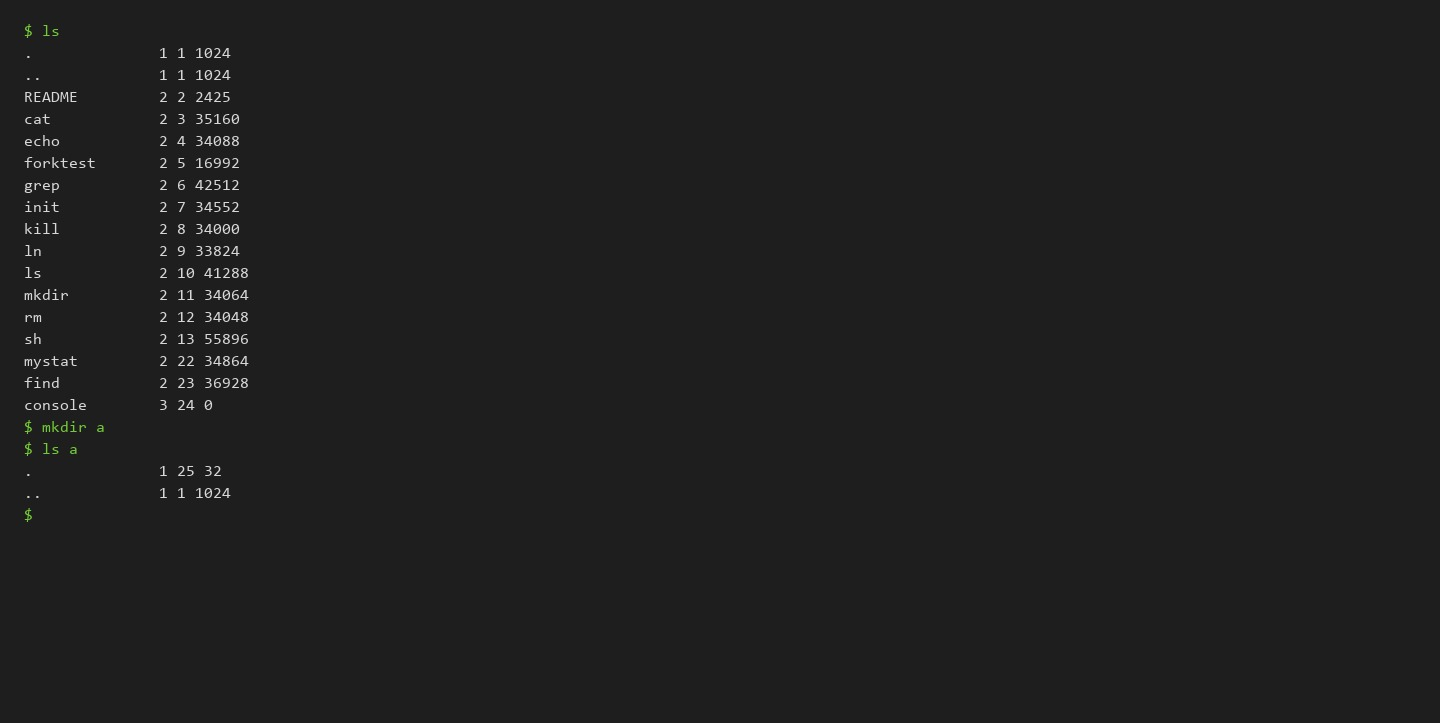
\includegraphics[width=0.92\textwidth]{assets/fig1_xv6_ls.jpg}
\caption{Reconstructed terminal illustration (not an original capture): directory listing and type decoding in xv6.}
\label{fig:l6_ls}
\end{figure}

\section{The Root Inode and Directory Self-Reference}
The root directory `/` is anchored at inode 1 (\texttt{ROOTINO = 1}). In every directory table, `.` references the directory itself, while `..` references its parent. Because the root directory has no parent above it, its parent entry points directly to itself. Both `.` and `..` therefore map to inode 1.

\section{Directory Record Sizing}
Directory entries are defined by \texttt{struct dirent} in \texttt{kernel/fs.h}:
\begin{verbatim}
struct dirent {
  ushort inum;         // 2 bytes
  char name[DIRSIZ];   // 14 bytes (DIRSIZ = 14)
};
\end{verbatim}
Each directory entry spans exactly 16 bytes. Creating an empty directory \texttt{a} yields:
\begin{verbatim}
$ mkdir a
$ ls a
.              1 25 32
..             1 1 1024
\end{verbatim}
The size of directory \texttt{a} is 32 bytes, consisting of exactly two 16-byte entries: `.` (inode 25) and `..` (inode 1).

\chapter{The mystat Utility and Hard Link Lifecycle}

\section{Implementation of user/mystat.c}
The \texttt{mystat} utility invokes \texttt{stat()} to print detailed object metadata. Figure \ref{fig:l6_links_concept} sketches the name-to-inode relationship used in this trace; it omits the open-file-table layer.

\begin{figure}[H]
\centering
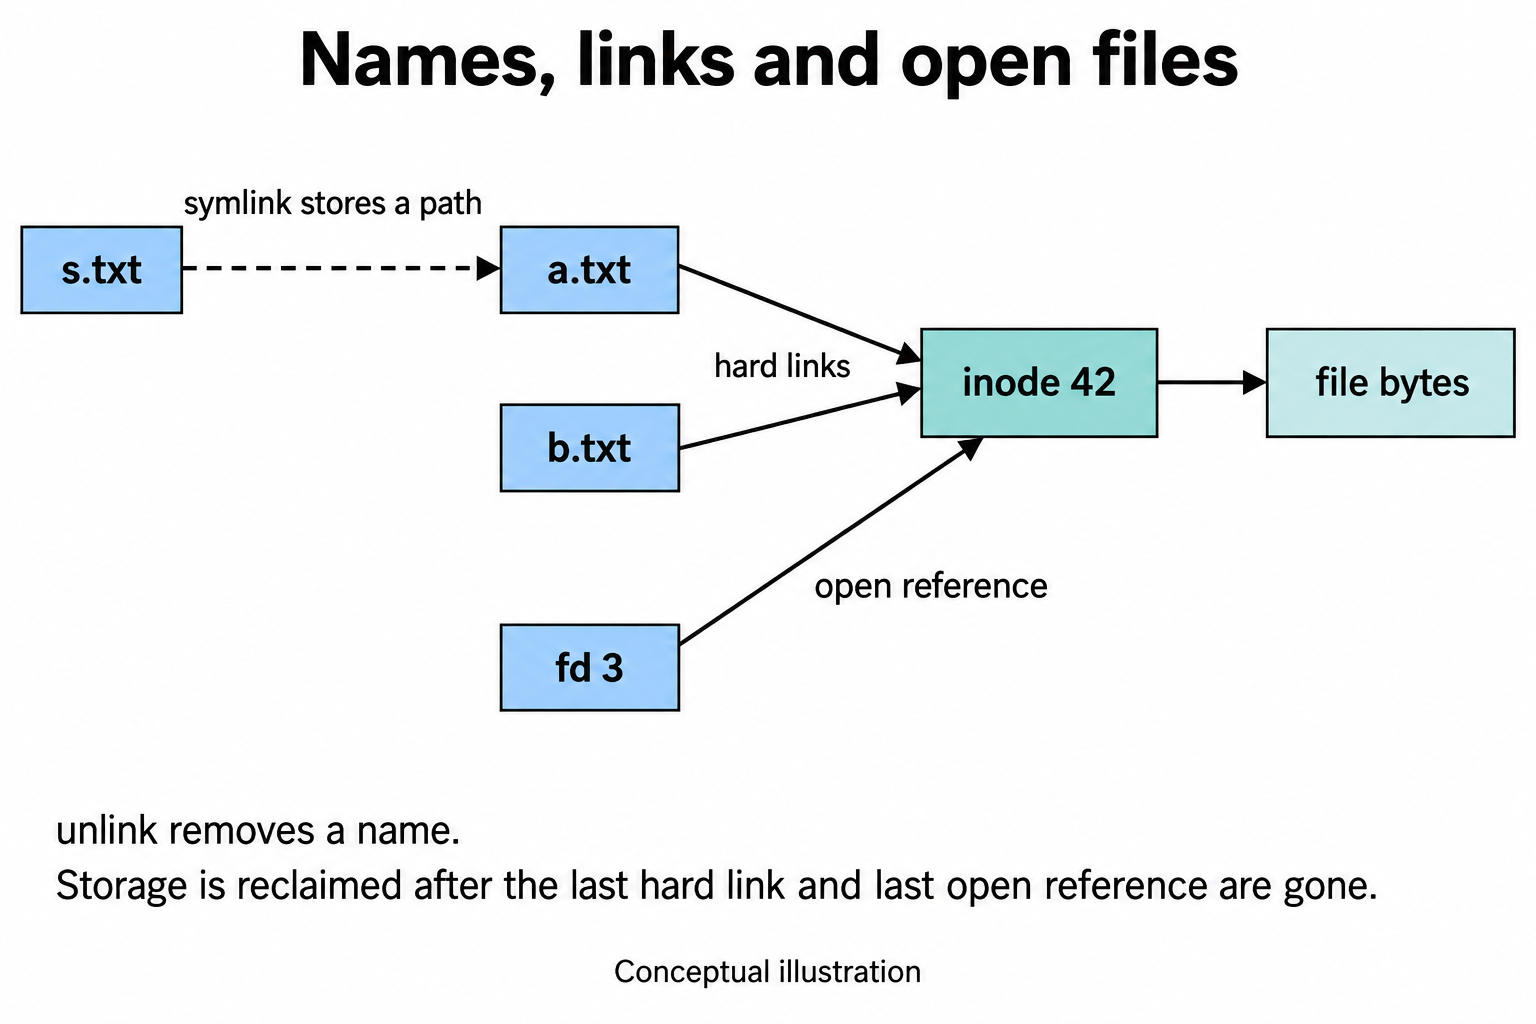
\includegraphics[width=0.88\textwidth]{assets/concept-filesystem-links.png}
\caption{Conceptual diagram of names, inodes, and links; the open-file-table layer is omitted. Generated illustration, not execution evidence.}
\label{fig:l6_links_concept}
\end{figure}


\begin{verbatim}
#include "kernel/types.h"
#include "kernel/stat.h"
#include "user/user.h"

char *typename(int t) {
  switch(t) {
  case T_DIR:    return "directory";
  case T_FILE:   return "file";
  case T_DEVICE: return "device";
  default:       return "?";
  }
}

int main(int argc, char *argv[]) {
  struct stat st;
  for(int i = 1; i < argc; i++){
    if(stat(argv[i], &st) < 0){
      fprintf(2, "mystat: cannot stat %s\n", argv[i]);
      continue;
    }
    printf("%s: %s, inode %d, links %d, size %ld bytes\n",
           argv[i], typename(st.type), st.ino, st.nlink, st.size);
  }
  exit(0);
}
\end{verbatim}

\section{Observing Hard Links and Unlinking}
\begin{verbatim}
$ mystat README . console
README: file, inode 2, links 1, size 2425 bytes
.: directory, inode 1, links 2, size 1024 bytes
console: device, inode 24, links 1, size 0 bytes

$ ln README r2
$ mystat README r2
README: file, inode 2, links 2, size 2425 bytes
r2: file, inode 2, links 2, size 2425 bytes

$ rm README
$ mystat r2
r2: file, inode 2, links 1, size 2425 bytes

$ cat r2 | wc
48 334 2425
\end{verbatim}

\begin{figure}[H]
\centering
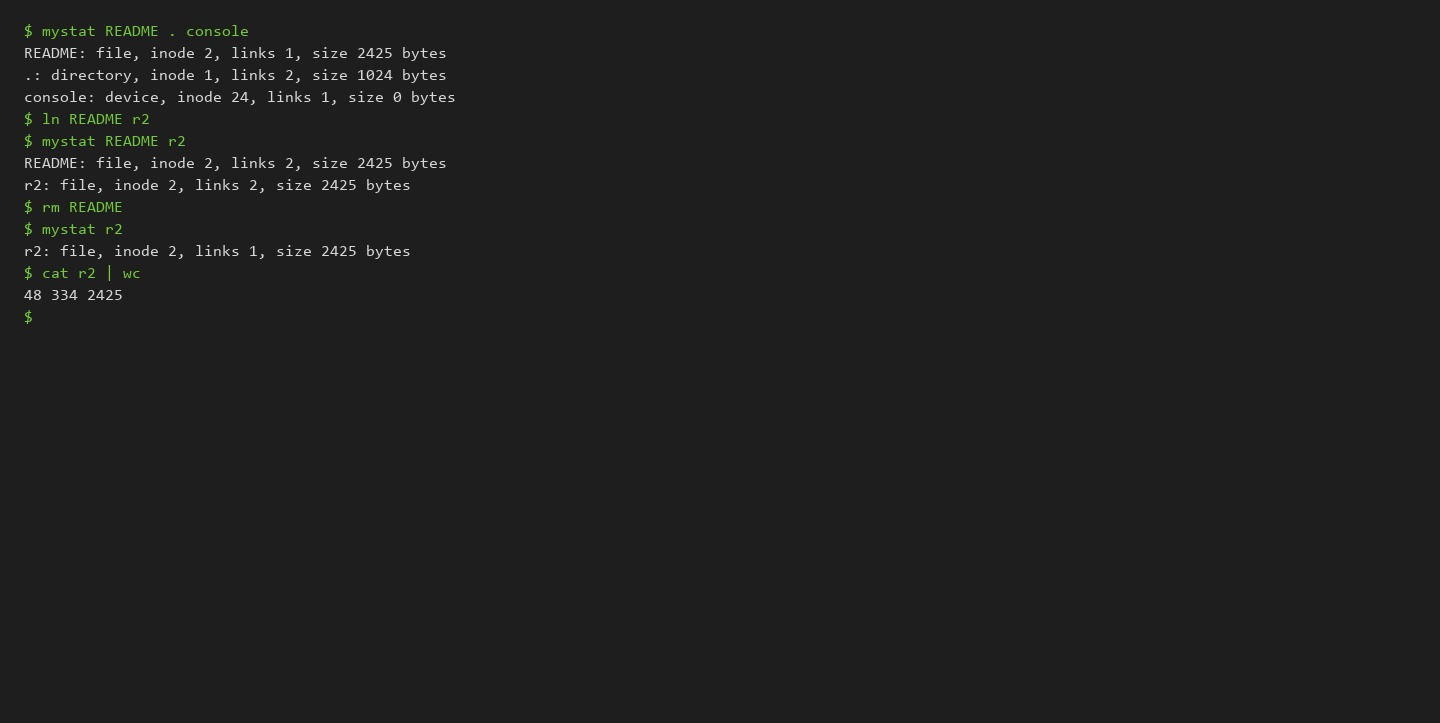
\includegraphics[width=0.92\textwidth]{assets/fig2_mystat_links.jpg}
\caption{Reconstructed terminal illustration (not an original capture): mystat output, link counter increment, and unlinking.}
\label{fig:l6_mystat_links}
\end{figure}

When \texttt{ln README r2} executes, the kernel creates a second directory entry referencing inode 2, incrementing \texttt{nlink} to 2. Inode number, size, and content remain identical. When \texttt{README} is removed, \texttt{sys\_unlink()} removes only the directory entry and decrements \texttt{nlink} back to 1. Inode 2 and its data blocks remain intact, allowing \texttt{r2} to read the original contents.

\section{Kernel Unlinking and Block Deallocation Tracing}
In \texttt{kernel/sysfile.c}, the hard link count is decremented at line 230:
\begin{verbatim}
ip->nlink--;
iupdate(ip);
\end{verbatim}
Crucially, \texttt{sys\_unlink()} does not free disk blocks. Block freeing is deferred to \texttt{iput()} in \texttt{kernel/fs.c} (line 342):
\begin{verbatim}
if(ip->ref == 1 && ip->valid && ip->nlink == 0){
  itrunc(ip);
  ip->type = 0;
  iupdate(ip);
  ip->valid = 0;
}
\end{verbatim}
Physical data blocks are freed only when the in-memory reference count drops to 1 and the on-disk link count drops to 0. At that point, \texttt{itrunc()} iterates across all direct and indirect block addresses, calling \texttt{bfree()} to return blocks to the free bitmap.

\section{Minimalist On-Disk Inode Structure}
The on-disk inode structure (\texttt{struct dinode} in \texttt{kernel/fs.h}) illustrates xv6's minimalist design:
\begin{verbatim}
struct dinode {
  short type;              // File type
  short major;             // Major device number (T_DEVICE only)
  short minor;             // Minor device number (T_DEVICE only)
  short nlink;             // Hard link counter
  uint size;               // File size in bytes
  uint addrs[NDIRECT+1];   // Block addresses (12 direct + 1 indirect)
};
\end{verbatim}
xv6 omits permission bits, UID, GID, timestamps, and symbolic link paths.

\chapter{Filesystem Limits and Disk Layout}

\section{Structural Constants in kernel/fs.h}
\begin{verbatim}
$ grep -n "define BSIZE\|define NDIRECT\|define NINDIRECT\|define DIRSIZ" kernel/fs.h
6:#define BSIZE 1024  // block size
27:#define NDIRECT 12
28:#define NINDIRECT (BSIZE / sizeof(uint))
54:#define DIRSIZ 14
\end{verbatim}

\section{Name Truncation}
Creating a directory whose name exceeds 14 characters reveals truncation:
\begin{verbatim}
$ mkdir averyveryverylongname
$ ls
averyveryveryl 1 26 32
\end{verbatim}

\begin{figure}[H]
\centering
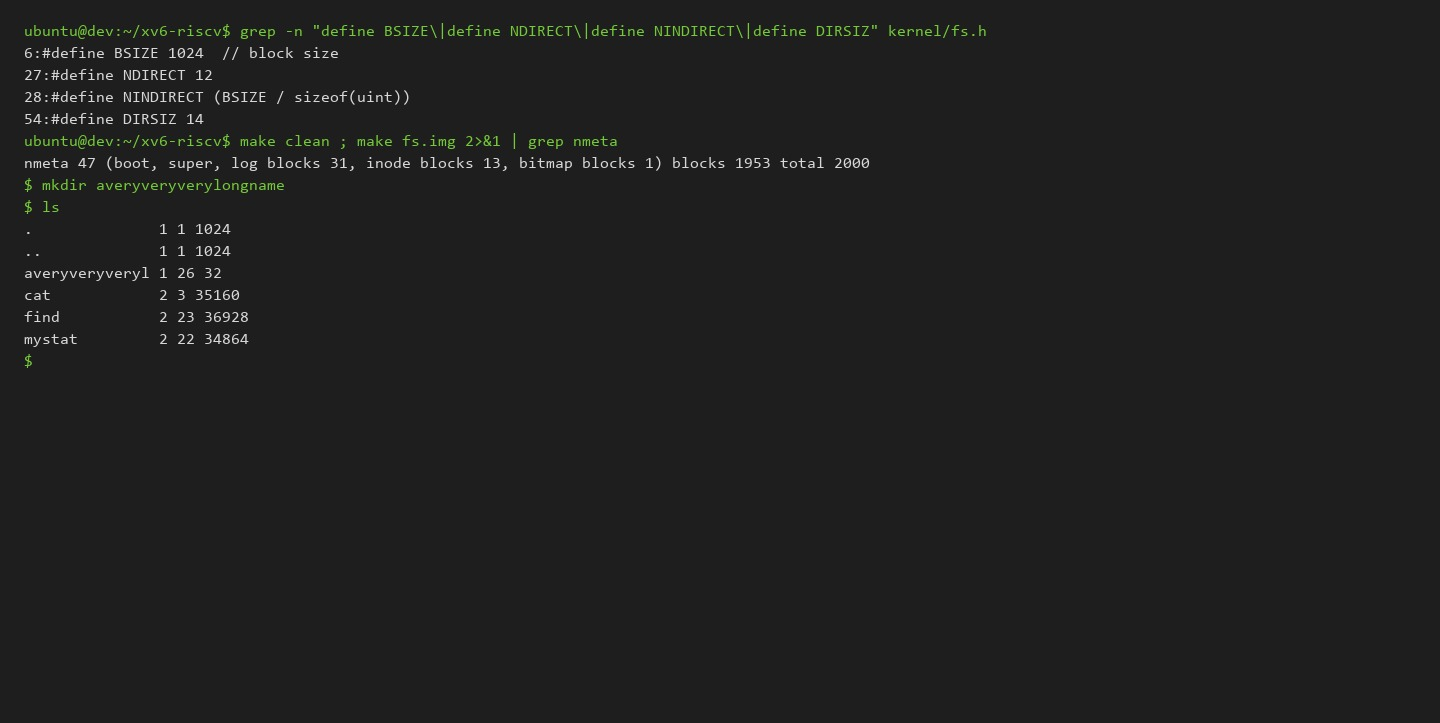
\includegraphics[width=0.92\textwidth]{assets/fig3_limits_truncation.jpg}
\caption{Reconstructed terminal illustration (not an original capture): measuring constants, disk layout, and 14-byte truncation.}
\label{fig:l6_limits}
\end{figure}

Because \texttt{DIRSIZ = 14}, names are truncated to 14 characters within the directory entry buffer.

\section{Maximum File Capacity Calculation}
\begin{itemize}
\item Block size: $\text{BSIZE} = 1024\text{ bytes}$;
\item Direct blocks: $\text{NDIRECT} = 12$ blocks ($12 \times 1024 = 12,288\text{ bytes}$);
\item Indirect blocks: $\text{NINDIRECT} = \frac{\text{BSIZE}}{\text{sizeof}(\text{uint})} = \frac{1024}{4} = 256$ block pointers ($256 \times 1024 = 262,144\text{ bytes}$);
\item Total blocks: $12 + 256 = 268$ blocks;
\item Maximum file size: $268 \times 1024\text{ bytes} = 274,432\text{ bytes} \approx 268\text{ KiB}$;
\end{itemize}

\section{Disk Layout from mkfs}
\begin{verbatim}
nmeta 47 (boot, super, log blocks 31, inode blocks 13, bitmap blocks 1) blocks 1953 total 2000
\end{verbatim}
The virtual disk spans 2000 blocks (2 MiB). Metadata consumes 47 blocks (block 0 boot, block 1 super, blocks 2--31 log, blocks 32--44 inodes, block 45 bitmap). The remaining 1953 blocks are allocated for user data.

\chapter{Recursive Search: user/find.c and Stretch}

\section{Implementation Architecture}
The \texttt{find} utility opens directory file descriptors, scans \texttt{struct dirent} entries, skips `.` and `..` to prevent cycles, formats paths in a local buffer, and recurses into subdirectories while strictly closing descriptors:

\begin{verbatim}
#include "kernel/types.h"
#include "kernel/stat.h"
#include "user/user.h"
#include "kernel/fs.h"
#include "kernel/fcntl.h"

static int show_ino = 0;

void find(char *path, char *target) {
  char buf[512], *p;
  int fd;
  struct dirent de;
  struct stat st;

  if((fd = open(path, O_RDONLY)) < 0) return;
  if(fstat(fd, &st) < 0 || st.type != T_DIR) { close(fd); return; }

  strcpy(buf, path);
  p = buf + strlen(buf);
  *p++ = '/';

  while(read(fd, &de, sizeof(de)) == sizeof(de)){
    char name[DIRSIZ + 1];
    if(de.inum == 0) continue;
    memmove(name, de.name, DIRSIZ);
    name[DIRSIZ] = 0;
    if(strcmp(name, ".") == 0 || strcmp(name, "..") == 0) continue;

    strcpy(p, name);
    if(stat(buf, &st) < 0) continue;
    if(strcmp(name, target) == 0){
      if(show_ino) printf("%s %d\n", buf, st.ino);
      else printf("%s\n", buf);
    }
    if(st.type == T_DIR) find(buf, target);
  }
  close(fd);
}
\end{verbatim}

\section{Validation and Inode Identity Verification}
\begin{verbatim}
$ mkdir a
$ mkdir a/b
$ echo x > a/b/r2
$ echo y > a/r2
$ ln cat r2

$ find . r2
./r2
./a/b/r2
./a/r2

$ find a b
a/b

$ find . r2 -n
./r2 3
./a/b/r2 26
./a/r2 27

$ mystat cat
cat: file, inode 3, links 2, size 35160 bytes
\end{verbatim}

\begin{figure}[H]
\centering
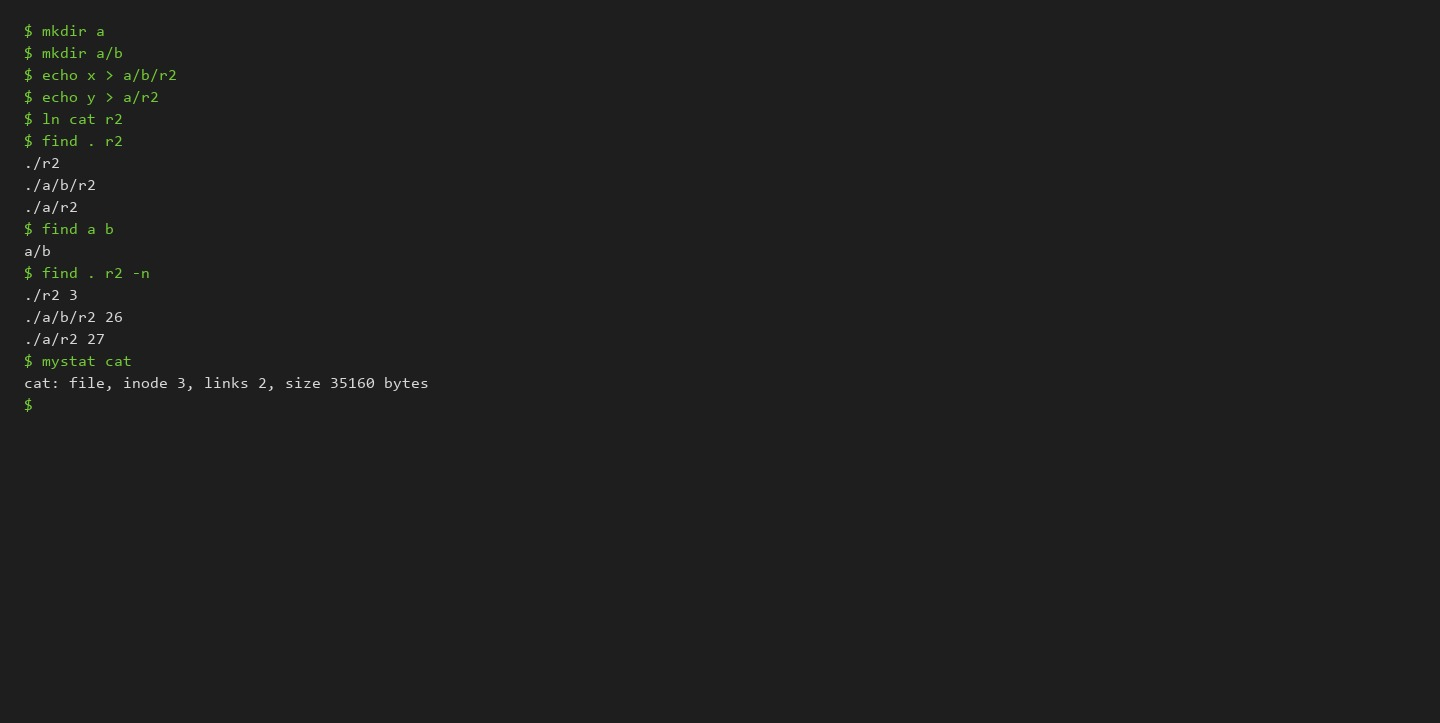
\includegraphics[width=0.92\textwidth]{assets/fig4_find_and_stretch.jpg}
\caption{Reconstructed terminal illustration (not an original capture): find output and -n inode comparison.}
\label{fig:l6_find_stretch}
\end{figure}

The saved stretch transcript reports that \texttt{./r2} (inode 3) and \texttt{cat} (inode 3, link count 2) share an inode. It also reports distinct inode numbers for \texttt{a/b/r2} (26) and \texttt{a/r2} (27); those values are specific to the recorded image.

\utmconclusions
Source analysis shows how directory names map to inodes, how link counts affect inode lifetime, and how xv6 separates unlinking from block reclamation. The saved transcripts illustrate these mechanisms in one image; the available terminal-style figures are reconstructed illustrations, not original captures.

\appendix
\chapter{Fresh xv6 Execution, 23 October 2026}
\section{Environment and scope}
The captured session is preserved in \texttt{execution-2026-10-23.txt}. It ran in Ubuntu 24.04 WSL2 on the WSL2 Linux 6.18.33.2 kernel, using host GCC 13.3.0, GNU make 4.3, Perl 5.38.2, RISC-V GCC 13.2.0, and QEMU 8.2.2. The Lab 6 helper built a disposable overlay under \texttt{/tmp}. The linker emitted RWX-segment warnings for the kernel and \texttt{user/\_forktest}; QEMU/make exited with status 0, then the overlay was removed.

\section{Captured commands and output}
\begingroup
\footnotesize
\begin{verbatim}
$ mystat README . console
README: file, inode 2, links 1, size 2473 bytes
.: directory, inode 1, links 1, size 1024 bytes
console: device, inode 26, links 1, size 0 bytes
$ ln README r2
$ mystat README r2
README: file, inode 2, links 2, size 2473 bytes
r2: file, inode 2, links 2, size 2473 bytes
$ rm README
$ mystat r2
r2: file, inode 2, links 1, size 2473 bytes
$ mkdir a
$ mkdir a/b
$ echo x > a/b/r2
$ echo y > a/r2
$ find a r2
a/b/r2
a/r2
$ find a r2 -n
a/b/r2 28
a/r2 29
\end{verbatim}
\endgroup

This image shows README and r2 sharing inode 2, with the link count falling from two to one after unlink. find recursed through a/b and reported the two r2 inodes as 28 and 29. These numbers identify this image only; the run did not repeat the cat hard link or filesystem-limit observations.
\end{document}
